\documentclass[conference]{IEEEtran}
\ifCLASSINFOpdf
  \usepackage[pdftex]{graphicx}
  \graphicspath{{../pdf/}{../jpeg/}}
  \DeclareGraphicsExtensions{.pdf,.jpeg,.png}
\else
  \usepackage[dvips]{graphicx}
  \graphicspath{{../eps/}}
  \DeclareGraphicsExtensions{.eps}
\fi
\usepackage{cite}
\usepackage{times}
\usepackage[cmex10]{amsmath}
\usepackage{algorithmic}
\usepackage{array}
\usepackage[tight,footnotesize]{subfigure}
\usepackage{fixltx2e}
\usepackage{url}

\begin{document}

% paper title
\title{Iterative MIMO Detection for Large Wireless MIMO Systems}

% author names and affiliations
\author{
\IEEEauthorblockN{Alexandre P. J. Dixneuf}
\IEEEauthorblockA{Student, CentraleSupélec}
\and
\IEEEauthorblockN{Antoine Berthet}
\IEEEauthorblockA{Professor, CentraleSupélec}
}

% make the title area
\maketitle

\begin{abstract}
  In a large-scale network, it is common to encounter systems that require multiple transmitting antennas as well as multiple receiving antennas. These systems, referred to as Multiple-Input, Multiple-Output (MIMO) are the cornerstone of modern network architectures. Unfortunately, they add a higher level of complexity that makes basic decoding techniques either inaccurate or infeasible. This report will study five main variables that are both common to see in real-world applications, and each have a major impact on accurately receiving transmitted messages. These are the number of transmitting antennas, the number of receiving antennas, the number of time steps and thus messages sent in the same transmission, the level of encoding (M-QAM), and the signal-to-noise ratio (SNR). This report will study a variety of detection and decoding techniques for large-scale MIMO systems, and will compare and contrast how each technique handles the change of each individual variable. First, both Belief Propagation (BP) and the Gaussian variant (GaBP) will be used as baselines. Then, a clustered approximation strategy will be employed using the same techniques. Lastly, Low-Density Parity-Check Codes (LDPCC) and Bit-Interleaved Coded Modulation (BICM) will both be implemented to enhance error correction and efficiency. Through simulations and performance analysis, the proposed implementations demonstrate potential improvements in complexity-performance tradeoffs, paving the way for scalable receiver architectures suitable for next-generation wireless networks such as 5G and beyond.
\end{abstract}

% Found this command online to force wey
\providecommand{\keywords}[1]{\textbf{\textit{Index terms---}}#1}
\begin{keywords}
\textbf{Massive MIMO, Belief Propagation, BP, Gaussian Approximation Belief Propagation, GaBP, Low-Density Parity-Check Codes, LDPCC, Bit-Interleaved Coded Modulation, BICM}
\end{keywords}

\IEEEpeerreviewmaketitle

\section{Introduction}
A basic transmission requires one side to send a message and one side to collect the message. In signal analysis, these are known as the transmitter and receiver. In the most basic of systems, a transmitter will prepare and send a message, and the receiver will simply receive the transmission. However, in real-world applications, there are fading effects and random noise which will muddy the signal. The first step to counter this would be to have a step amount of "acceptable" transmission, of which both sides know and agree on. Then, when the receiver receives the transmission, even if there is imperfection, the receiver will be able to see what is the closest "acceptable" transmission, and consider that to be the received signal. This, in essence, is the idea behind modulation and "nearest neighbor" decoding. For example, a signal that can only be a set of 0's and 1's means that, if the receiver observes [0.9, 0.1, 0.3, 0.7], they can conclude that the transmitter meant 1001. \par
One way to add complexity to the system would be to allow a larger range of values. For example, if we accept [0.0, 0.5, 1.0], then each symbol transmitted can be one of three values, rather than the previous one of two, and thus the same length of transmission contains 1.5x as much information. However, this has a weakness: it also means the margin of error is smaller. In the example with 0's and 1's, the transmission could have $\pm$ 0.5 and still be decoded without error. In the new example, this is lowered to $\pm$ 0.25, meaning half the margin of error for only one and half times the information. To demonstrate this, with our original transmission of [1.0, 0.0, 0.0, 1.0], if the receiver again detected [0.9, 0.1, 0.3, 0.7], it would instead be decoded as [1.00, 0.00, 0.50, 0.50], which has an accuracy of 50\%.\par
One method to overcome this is to increase the number of transmitting antennas. Rather than one antenna with three possible values, two antennas each with two possible values can each send less information with a less-strict modulation with better accuracy. In addition, more receiving antennas would mean random noise has less of an impact. Unfortunately, as these variables all keep changing, the "nearest neighbor" method becomes impractical in any real-world setting, and thus new techniques need to be investigated.\par
To address these challenges, this report focuses on iterative MIMO detection using probabilistic graphical models, particularly Belief Propagation (BP) and Gaussian Belief Propagation (GaBP), as a baseline framework. Building on this foundation, the study explores reduced-complexity strategies such as clustered Gaussian approximation and integrates advanced coding and modulation schemes like Low-Density Parity-Check Codes (LDPC) and Bit-Interleaved Coded Modulation (BICM). These techniques aim to provide near-optimal performance under realistic system constraints while maintaining manageable complexity. This report will focus on implementing each of these techniques with differing variables to see which technique suffers or thrives in which conditions.

\section{Background}
Large scale networks, such as cellular and local wireless networks, need to support a system of constantly changing users (both in count and location) over a large area for large quantities of data. Modern 4G and 5G networks use a technique known as multiple-output orthogonal frequency-division multiplexing (MIMO-OFDM). First developed by Greg Raleigh in 1996, this technique allows for multiple frequencies being used during the same transmission time, thus enabling a larger data throughput. However, more data means more complex decoding methods required. While merely one of many, the current study will review the problem of detection large number of (complex) signals taking values in finite alphabets.

\section{Theory}
\subsection{Belief Propagation (BP)}
A factor graph, as the name suggests, is a graphical representation of the factorization of a function. The main use of factor graphs is to assist in probabilistic calculations, especially over a large quantity of possibilities. There exists one major problem with using this method for decoding: the receiver has no knowledge of the transmission, and thus cannot use any calculation based on the transmission probability. Instead, a method known as Belief Propagation (BP) is used.\par
BP operates on factor graphs by passing messages between two types of nodes: variables and functions. By going through one direction and then the other over multiple iterations, the transmitted symbol vector is modeled as a set of discrete random variables, and the received signal defines a set of likelihood functions. Messages from variable to function nodes represent belief updates about variable values, while function-to-variable messages update those beliefs based on observed evidence and neighboring variables.

\subsection{Gaussian Belief Propagation (GaBP)}
GaBP is a variant of BP. BP depends on calculating individual distributions for each and every message. However, this means large quantities of data for each data point, and is the main reason why the following experiment will only be demonstrated with smaller-scale MIMO systems, as comparisons of accuracy would be impossible otherwise since the BP algorithm would have a lack of memory. To use less data, by treating every probability as a Gaussian distribution, we can use previous knowledge to use more computations and less memory. A Gaussian distribution is perfectly known using both a mean and variance, so storing these two values will be enough to replicate the distribution. This allows a significant reduction in complexity and enables simpler updates between iterations.

\subsection{Clustered Gaussian Approximation}
Again simplifying the calculations, by grouping data points together, it is possible to run fewer but more complicated calculations. The exact size of each cluster can be altered with varying results, with a trade-off between accuracy and complexity. This is also known as the Group-wise Gaussian Approximation, although this report will remain with the name Clustered.

\subsection{Low-Density Parity-Check Codes}
Low-Density Parity-Check Codes (LDPCC) are linear block codes represented by sparse bipartite graphs and decoded using iterative BP. Each and every bit can be individually mapped to modulated symbols, allowing for a far more resilient system. However, it includes a large increase in complexity, especially when dealing with large modulations (large values of M).

\subsection{Bit-Interleaved Coded Modulation}
Bit-Interleaved Coded Modulation (BICM) combines channel coding and channel modulation. By interleaving each of the coded bits before mapping them onto modulation symbols, we can increase the diversity by spreading consecutive bits over different symbols, making the system far more robust to error.

\section{Reasoning}
Each of the techniques mentioned have their reason for being implemented in a MIMO system. Using full BP gives a solid starting point, but its computational cost grows quickly as the number of antennas and users increases. Therefore, it is no longer acceptable in a large-scale MIMO system. We can lower this complexity by invoking Gaussian belief propagation (GaBP) by assuming the variables follow Gaussian distributions — an assumption that often holds in large systems or after enough averaging. After all, each user will have their own message to send, and with enough users and enough message contents almost every system averages out to at least resemble a Gaussian system.\par
However, this is still an assumption and it not perfect. Therefore, a clustered approach is used to simplify only parts of the system. By breaking the problem into manageable chunks where the Gaussian methods holds, a more accurate model can be implemented only where it matters. This hybrid approach strikes a good balance between accuracy and efficiency.

Finally, adding LDPCC and BICM completes the modern MIMO receiver setup. LDPCC give strong error correction with reasonable complexity, and BICM improves performance at the modulation level by making the system more robust and diverse. Combined, these pieces create a flexible and high-performing receiver design that can be adjusted based on system needs.

\section{Methods}
To run the necessary simulations, several criteria had to be met. To begin, an overall network simulation needed to be created. This simulation must handle the creation of a random signal, the propagation of the signal through a channel, and then the easy manipulation and handling of the necessary data and problem parameters. Then, a basic decoder is necessary to allow for easy addition of decoders. Since the average user will use completely different frameworks for any and all codes, the simulation uses a virtual class Decoder which handles most of the data. This allows new decoder classes to simply override the virtual decode function to properly run, and thus new decoders can be added in the future for proper comparison. Lastly, the individual decoders analyzed throughout this report were implemented.

\subsection{General Structure}
The simulation depends on the use of a storage class called ProblemParameters. The simulation of transmitted signals in a MIMO system depends on multiple variables, such as the number of transmitting antennas, receiving antennas, the degree of modulation, the number of time steps and/or the signal-to-noise ratio. The variables all have different constraints, including non-negativity and the modulation required to be a power of 4. To avoid constant checks to avoid errors and bugs, all of the data is stored in the storage class ProblemParameters. The class’s task is to verify the parameters given are acceptable and to convert everything to constants such that they may no longer be altered. It also keeps a constant structure so that every future component knows the proper steps to handle the data.
The next component is the class MySignal. This class is similar to the ProblemParameters in that it has the main purpose of being a robust storage class. Rather than trusting the user to know what format the signal should be, it forces a constant format, and verifies the accuracy and altering of the contained data. It also serves to generate the random signal, although it does mean it would require additional steps to run the simulation on given data rather than random data. While this will have no effect on the study’s result, it does hurt any future application of this code.
The next class is QAMConstellation. This class serves to independently handle the M-QAM modulation of signals, as well as receiving and drawing the proper gray code constellation.
Lastly, there remains the Channel class. This class handles taking the data, generating the channel conditions, and propagating the given signal through the channel.

\subsection{Virtual Decoder}
One of the guiding principles behind the structure of the code in this project is to ensure that future decoders can be easily added and thus compared to the current methods. To this purpose, a virtual Decoder class was developed. This class handles taking in any data that a decoder could use, all the while keeping the rest of the data still accessible in case of non-standard decoders. Then, it handles the majority of the work necessary for a C++ class. It leaves only the function "decode" virtual such that overriding classes only need to override the single function to be fully compatible. 

\subsection{Belief Propagation Decoder}
The Belief Propagation decoder operates on a probabilistic factor graph representation of the MIMO system. For each time step, messages are iteratively passed between variable nodes (representing transmitted symbols) and factor nodes (representing received signals). These messages contain log-probabilities (chose to avoid overly large or small values), allowing for numerical stability and easier normalization. The algorithm evaluates every possible symbol combination for all but one transmitter (exponentially many in $M^(N_t - 1)$), which severely limits scalability but allows for exact marginal inference in small systems. Each iteration updates beliefs based on received signals and current symbol estimates, with convergence refined over 10 iterations. Finally, symbol estimates are selected using a maximum a posteriori (MAP) rule based on the aggregated log-messages. While accurate for small-scale MIMO, the algorithm's complexity grows rapidly and makes it impractical for large systems. Unfortunately, this decoder heavily weakened most of the other simulations, as there was no point in running comparison simulations without comparison between methods, but this method failed at very small variable values. In a future lab it would be suggested to remove this one from the baseline results and merely start at GaBP.

\subsection{Gaussian Approximation Belief Propagation Decoder}
The Gaussian Approximation Belief Propagation (GaBP) decoder simplifies standard BP by assuming all messages follow Gaussian distributions. This drastically reduces memory requirements and computation time, replacing full probability distributions with just mean and variance for each transmitted symbol. At each iteration, the decoder refines its estimates by computing residuals at the receivers, subtracting interference from other transmitters. Using the known noise variance and current symbol estimates, updated means and variances are computed and propagated through the system. Unlike full BP, GaBP avoids exhaustive symbol enumeration, making it viable for larger MIMO systems, though it sacrifices some accuracy due to the Gaussian assumption.

\subsection{Clustered (Group-Wise) Decoder}
The Clustered Decoder, applies the GaBP framework to small, manageable subgroups of transmit antennas. At each iteration, the decoder selects clusters of fixed size (currently set to 4 symbols) and solves a local linear system to refine mean estimates for the symbols in that group. All symbols outside the current cluster are treated as interference and subtracted from the received signal, effectively reducing the system into a lower-dimensional subproblem. After processing all clusters, the full symbol estimate is updated. This allows for lower memory usage and better scalability than full BP, with higher accuracy than standard GaBP due to localized exact updates. Once all iterations are completed, each estimated symbol is mapped to the nearest constellation point. The fixed cluster size introduces a trade-off between efficiency and fidelity, making this approach especially useful when full-scale exact inference is computationally prohibitive.\par
This current experiment had a set group-size to ease the comparison between methods. Further testing should be conducted to see if adjusting this value would be beneficial or harmful.

\subsection{Low-Density Parity-Check Code Decoder}
The LDPCC decoder integrates channel decoding directly into the detection process by using a sparse parity-check matrix to perform iterative belief updates on bit-level log-likelihood ratios (LLRs). Each QAM symbol is first mapped to its binary representation using a Gray code mapping. Initial LLRs are computed based on the estimated distance between the received signal and each possible constellation point. These values serve as priors for message passing between variable and check nodes in the LDPC graph. Over multiple iterations, messages are updated using the standard min-sum approximation (based on hyperbolic tangent functions) to gradually enforce parity constraints and reduce bit errors. Once message passing converges, final bit decisions are made and mapped back to symbols. While offering strong error correction, this implementation suffers from compatibility and complexity issues in large-scale MIMO, partially due to bit-level operations being shoehorned into a symbol-level simulation framework.\par
This method appears to have the most difficulty running, most likely due to poor implementation, and is another reason why the results will be shown in small experiement sizes. Larger experiment continuously show either infinitely large computation times, or simply crashes and thus no computation. Should any reader wish to test to attached code, it may be beneficial to remove the test for LDPCC to ease the computation.

\subsection{Bit Interleaved Constellation Modulation Decoder}
The Bit-Interleaved Coded Modulation (BICM) decoder operates at the bit level by evaluating the log-likelihood ratios (LLRs) for each individual bit position of the transmitted QAM symbols. For each transmit antenna and time step, the decoder computes LLRs by marginalizing over all constellation symbols whose bit representations contain either a 0 or 1 at the targeted position. This is done using a soft metric derived from the Euclidean distance between the received signal and the reconstructed signal for each symbol. Once all bit LLRs are computed, a hard decision selects the symbol whose bits best align with the LLR signs. While this approach increases robustness to channel noise through bit-level diversity, it is computationally expensive and somewhat misaligned with a symbol-centric framework. As a result, the implementation suffers in performance unless properly integrated into a full iterative detection-decoding pipeline.

\section{Experiments and Results}
There are five independent variables being verified during this project: the number of transmitting antennas, the number of receiving antennas, the number of messages sent, the level of modulation (M-QAM), and the signal-to-noise ratio (SNR) of the transmitted signal. It would be impossible to test every combination of every variable to receive usable data, so a base framework was used. In "base" conditions, there are two transmitting and receiving antennas each, only two messages are sent in 16-QAM with an SNR of 20. Then, each variable indepently will be selected, going from a given minimum and maximum value while the ramaining vatiables are set to constantly be at the base conditions. Lastly, all algorithms that involve a number of iterations was given exactly 10 iterations. To allows for direct comparison between each variable and the resulting accuracy of the decoders.

\subsection{Transmitting Antennas}
The transmitting antenna can be considered the most constraining variable, as most decoding methods were unablet to handle anything past 5 transmitting antennas. Therefore, the range of tested values was from 2 antennas to 5 antennas, enough to get a general understanding of the relation between the number of antennas and the overall accuracy, without spending several days per simulation.
\begin{figure}[h!]
    \centering
    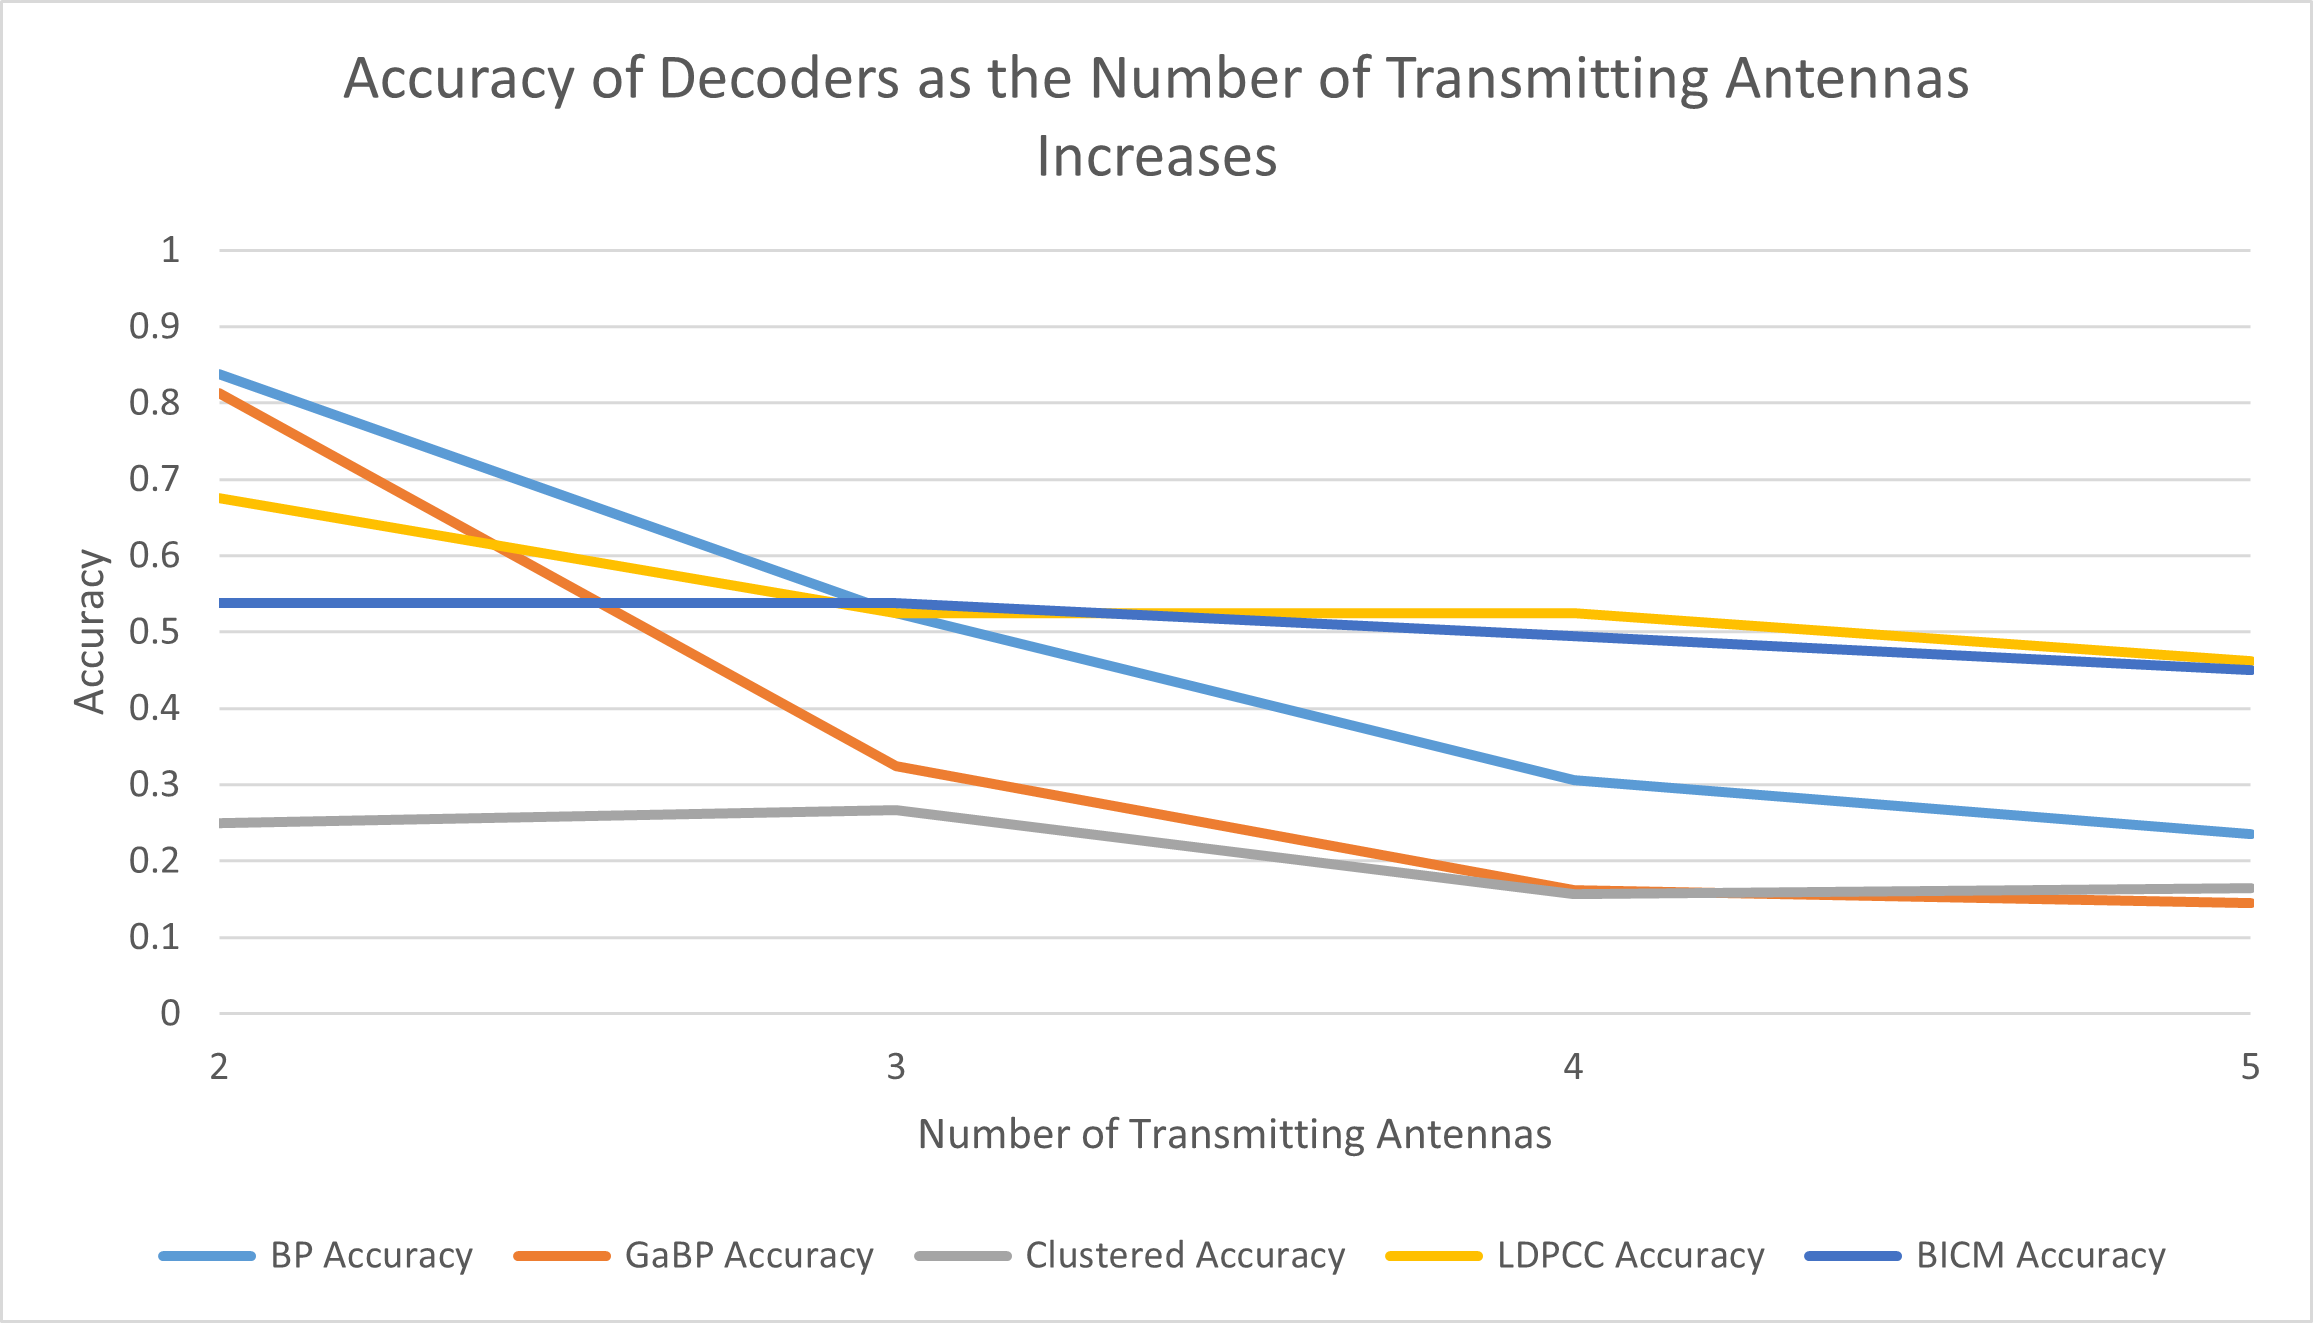
\includegraphics[width=0.30\textwidth]{NtGraph.png}
    \caption{A comparison of the accuracy of the various decoders as the number of transmitting antennas increases.}
    \label{fig:NtGraph}
\end{figure}

\subsection{Receiving Antennas}
The receiving antennas were much less constraining than the receiving antennas, and thus a larger range should have been possible, with original testing using 2 to 10. However, to keep the data uniform between experiments, the smaller range of tranmitting antennas, 2 to 5, was kept.
\begin{figure}[h!]
    \centering
    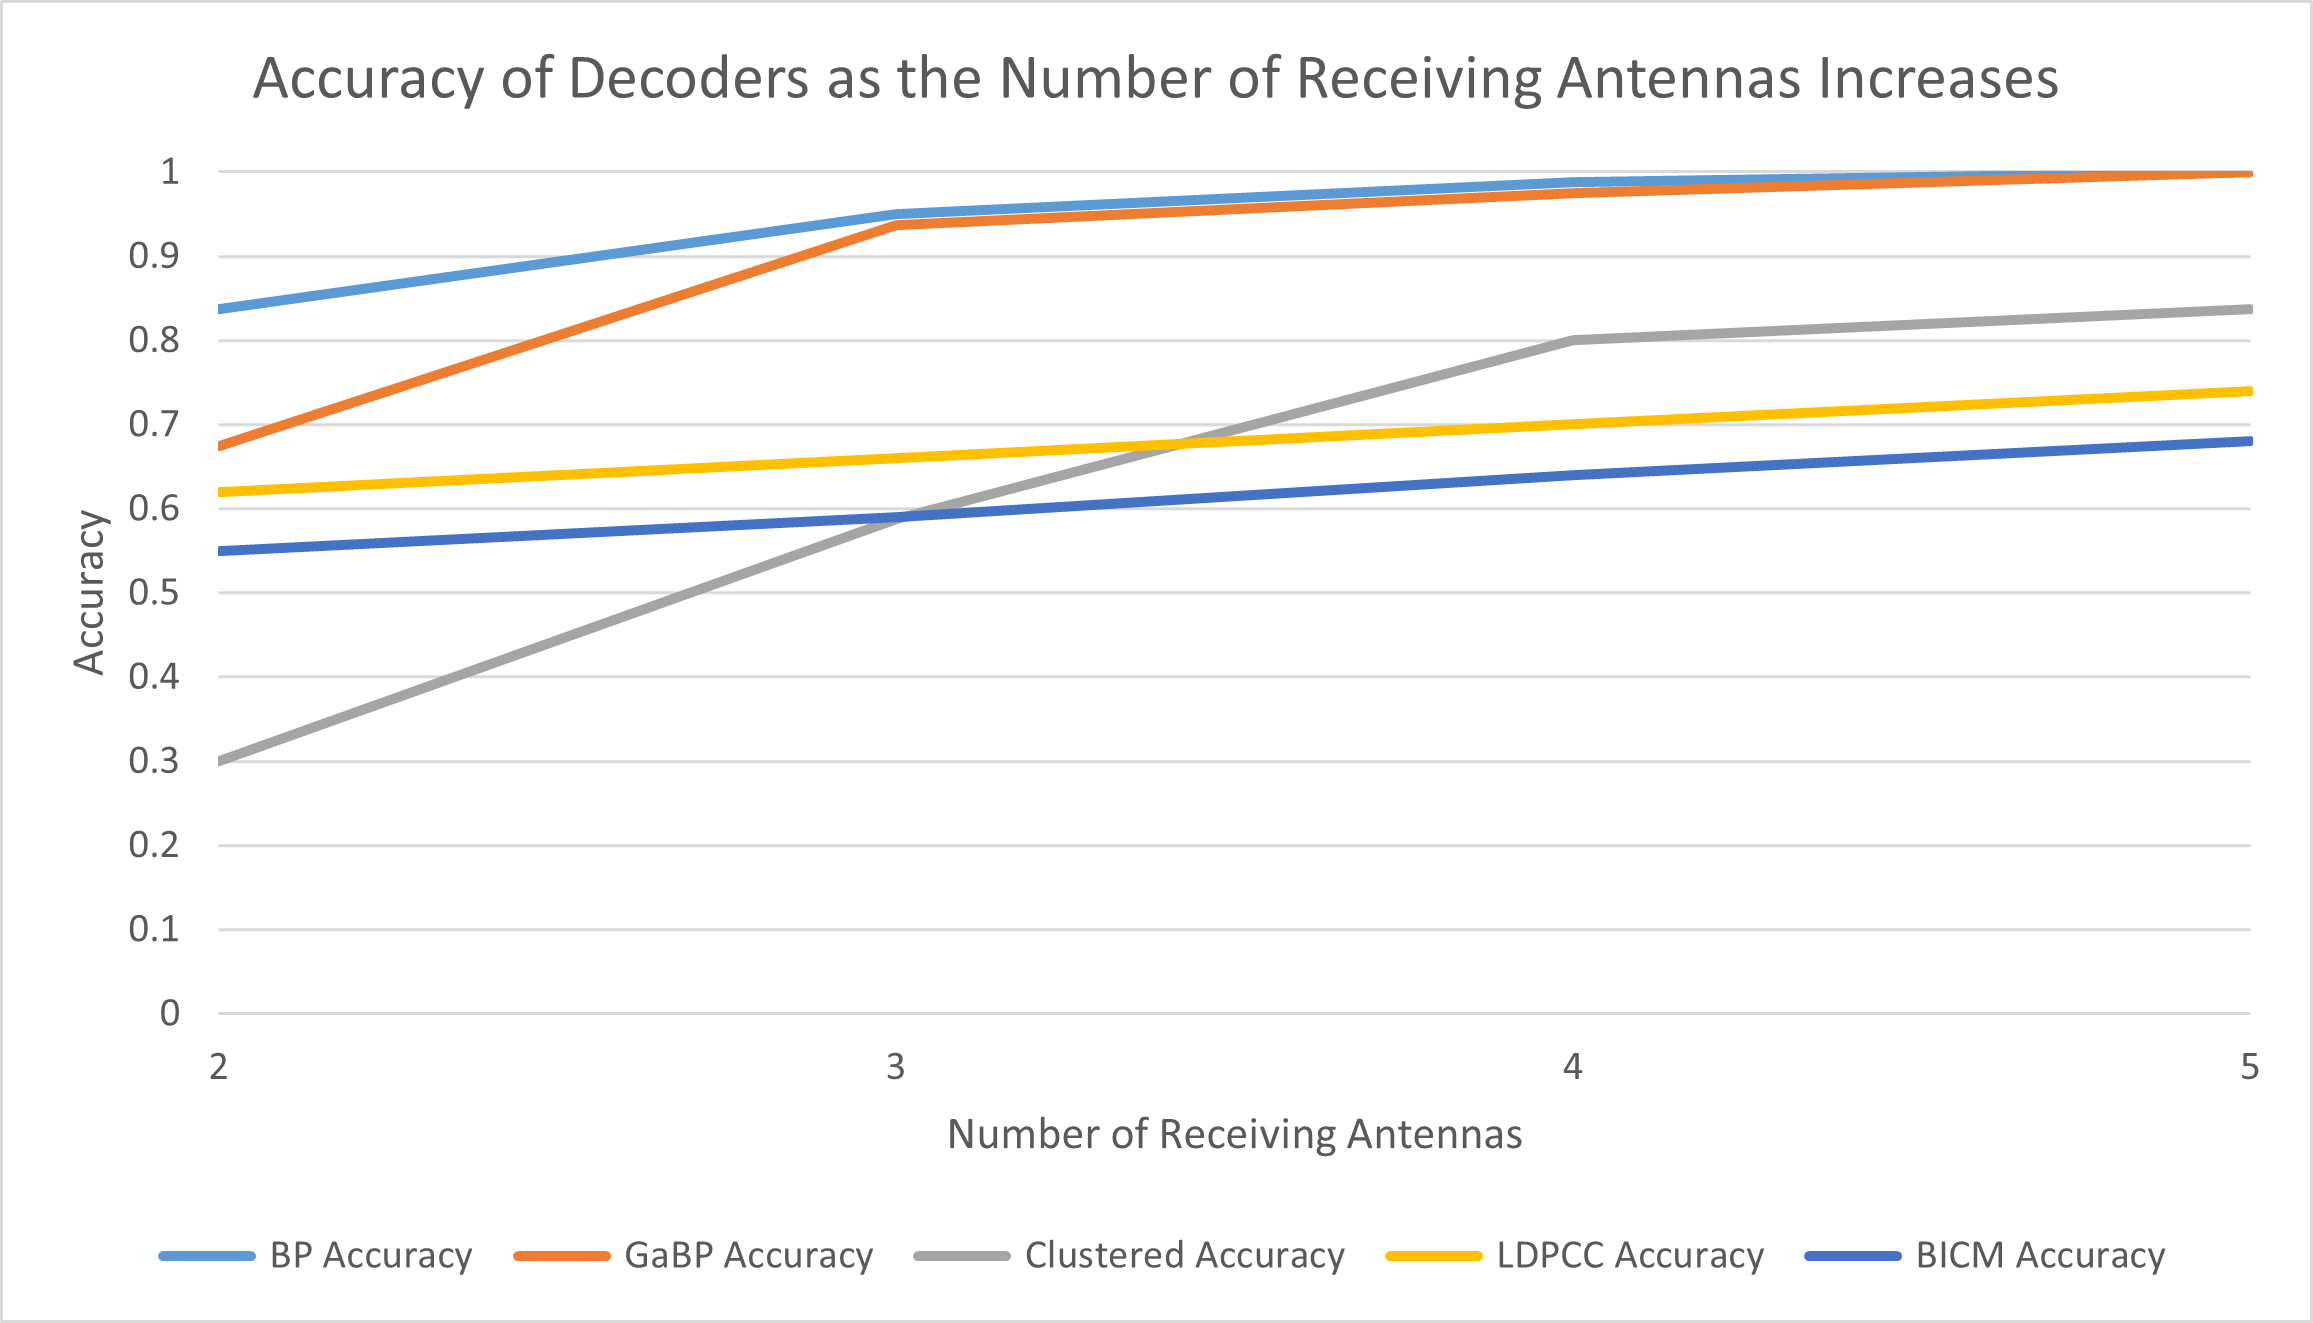
\includegraphics[width=0.30\textwidth]{NrGraph.png}
    \caption{A comparison of the accuracy of the various decoders as the number of receiving antennas increases.}
    \label{fig:NrGraph}
\end{figure}

\subsection{Messages Sent}
Compared to the previous sections, the number of messages sent has very little effect on the overall complexity of the decoders. Instead, it only lengthened the length of the simulations. A larger range of values was therefore possible, and thus the minimum of 2 and maximum of 10 was used.
\begin{figure}[h!]
    \centering
    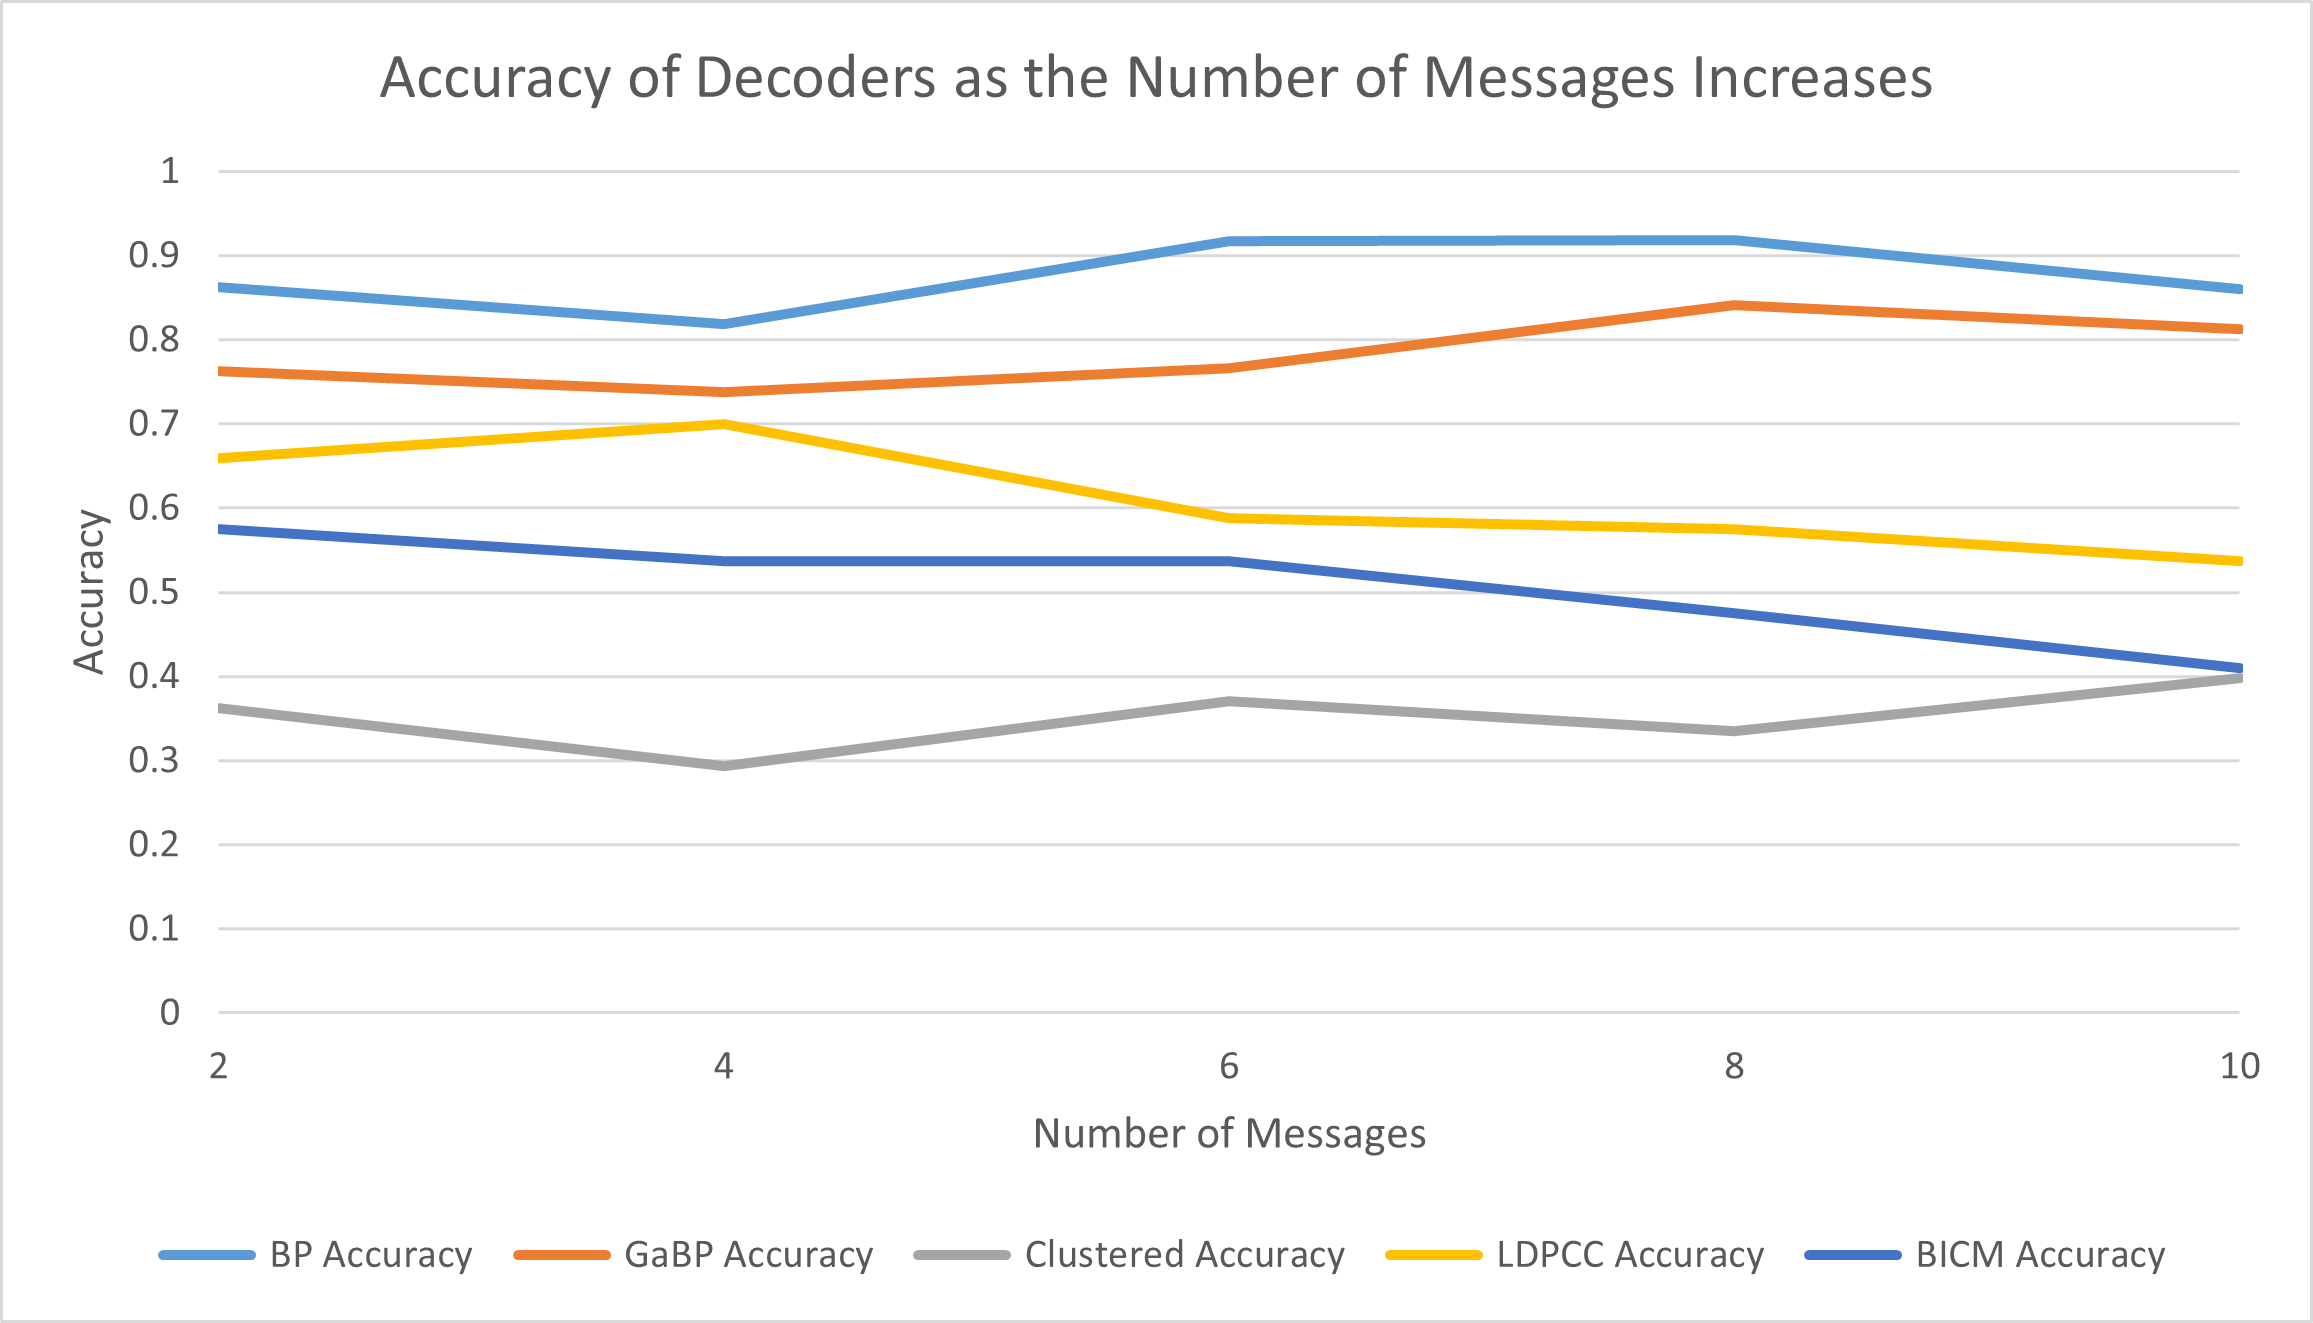
\includegraphics[width=0.30\textwidth]{TGraph.png}
    \caption{A comparison of the accuracy of the various decoders as the number of messages transmitted increases.}
    \label{fig:TGraph}
\end{figure}

\subsection{M-Modulation}
Testing values of M-QAM modulation was complicated, as only square constellations were possible to test, meaning values go from 4, to 16, then 64, 256, and then 1024. This means only 5 simulations change the complexity of the simulation by a factor of almost 1000. 1024 was too complicated and 4 gave no information as even a guess could have good decoding odds, so the values of 16-QAM, 64-QAM, and 256-QAM were used. While this gives minimal data, it should still give a rough idea of the relation.
\begin{figure}[h!]
    \centering
    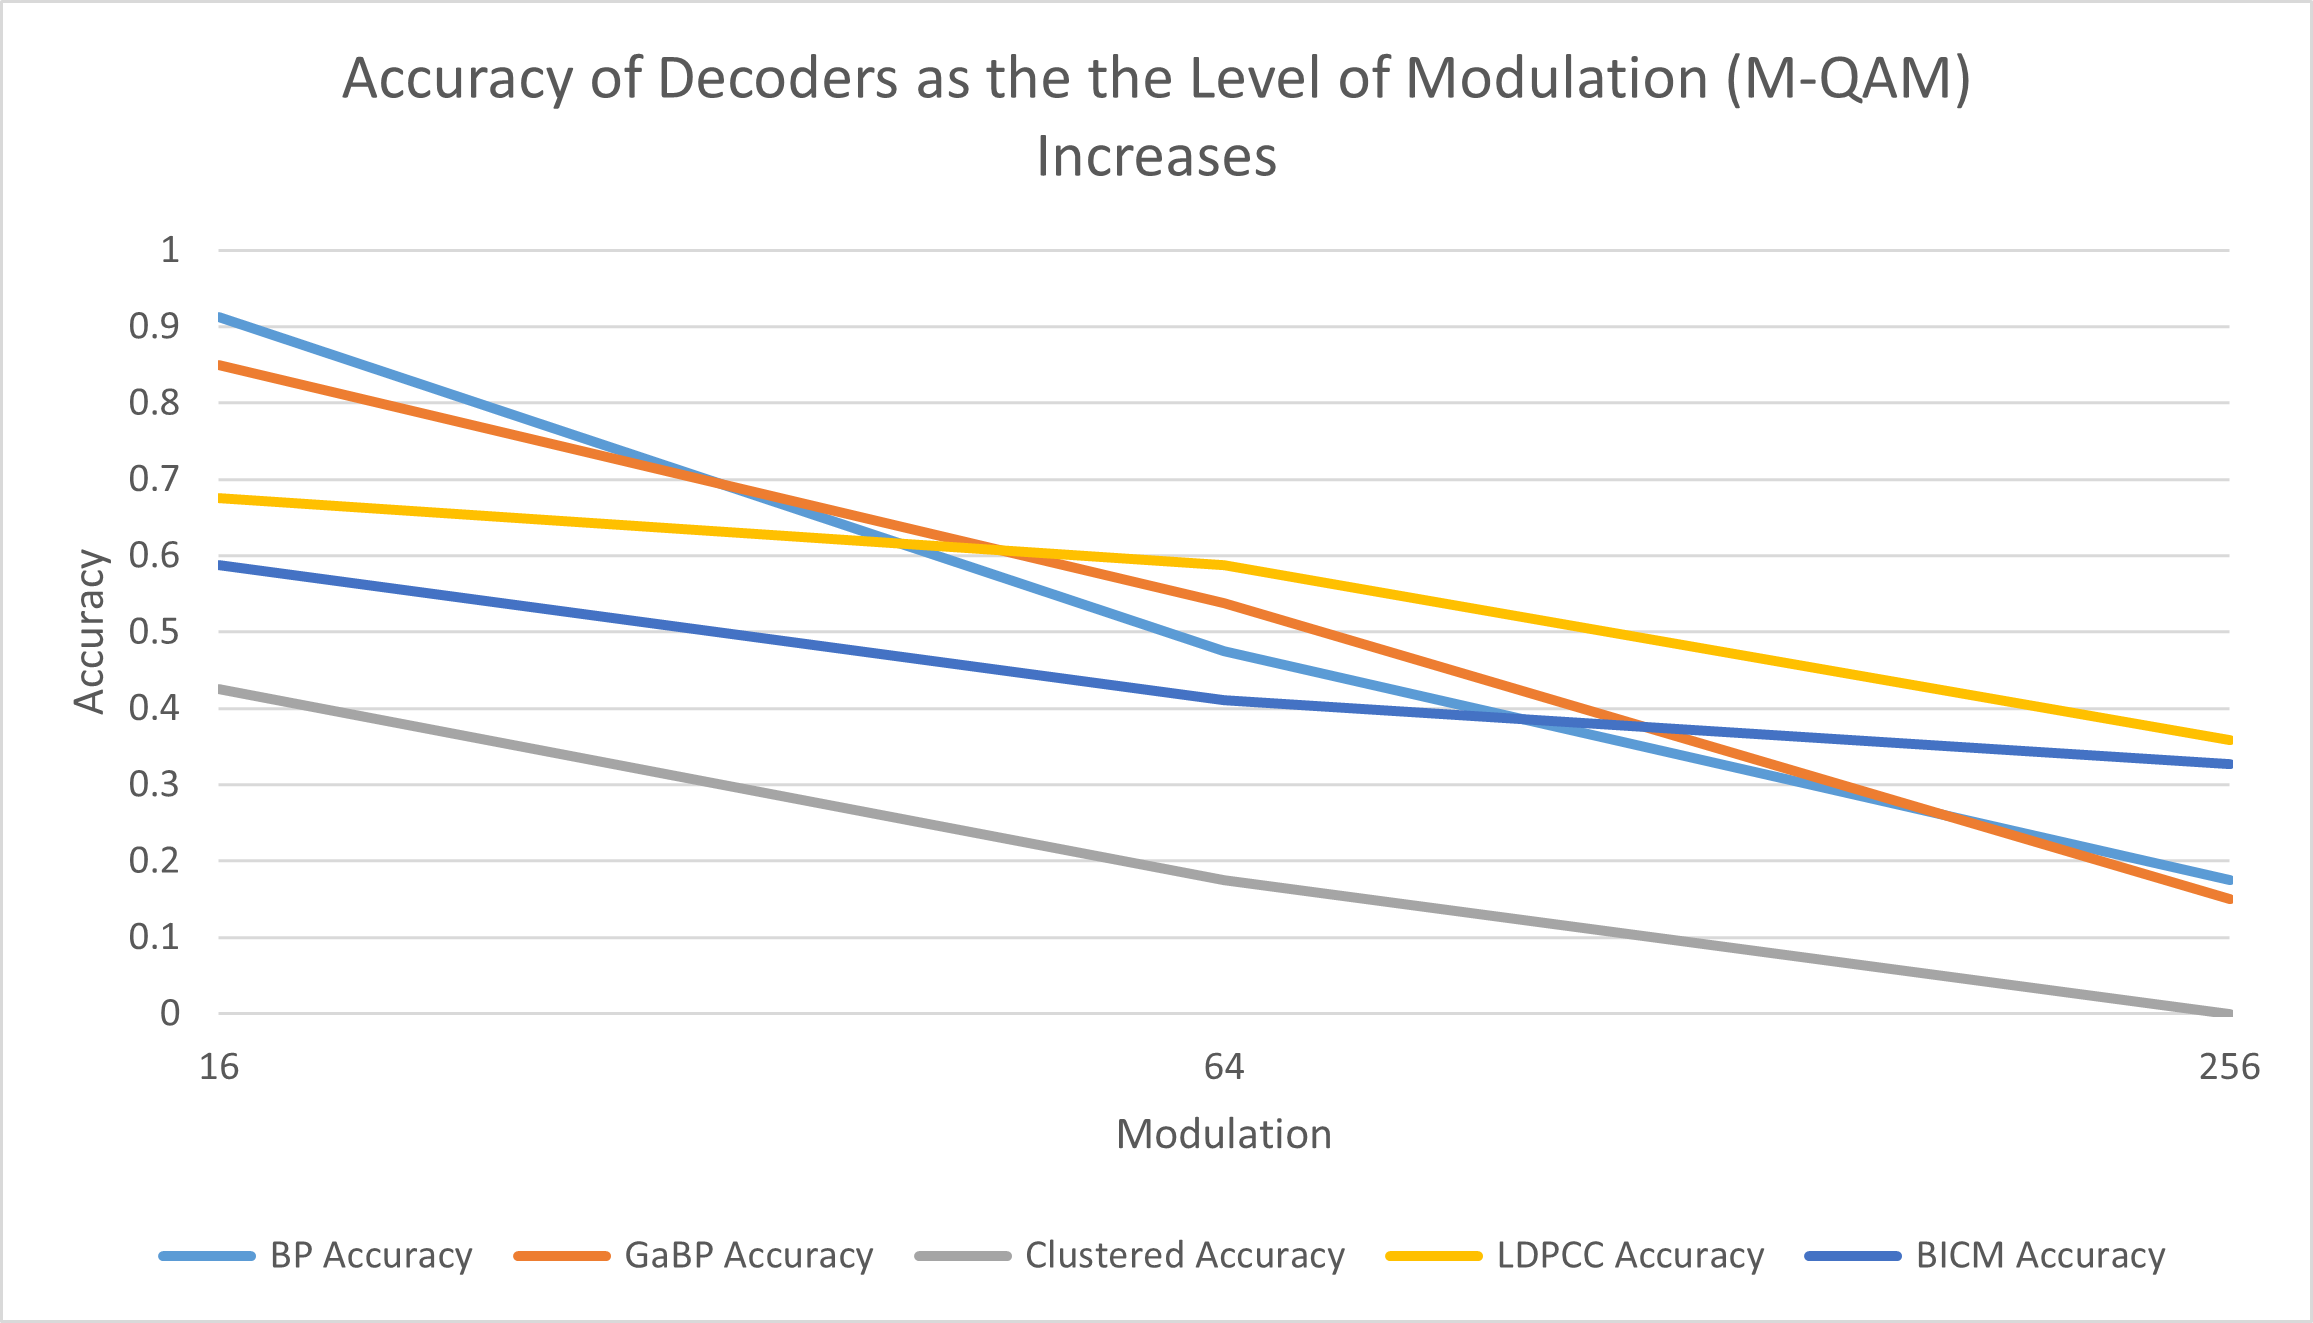
\includegraphics[width=0.30\textwidth]{MGraph.png}
    \caption{A comparison of the accuracy of the various decoders as the level of QAM modulation increases.}
    \label{fig:MGraph}
\end{figure}

\subsection{Signal-to-Noise Ratio}
The SNR has no effect on the complexity of the system, so a large range of 10 to 40 was able to be used.
\begin{figure}[h!]
    \centering
    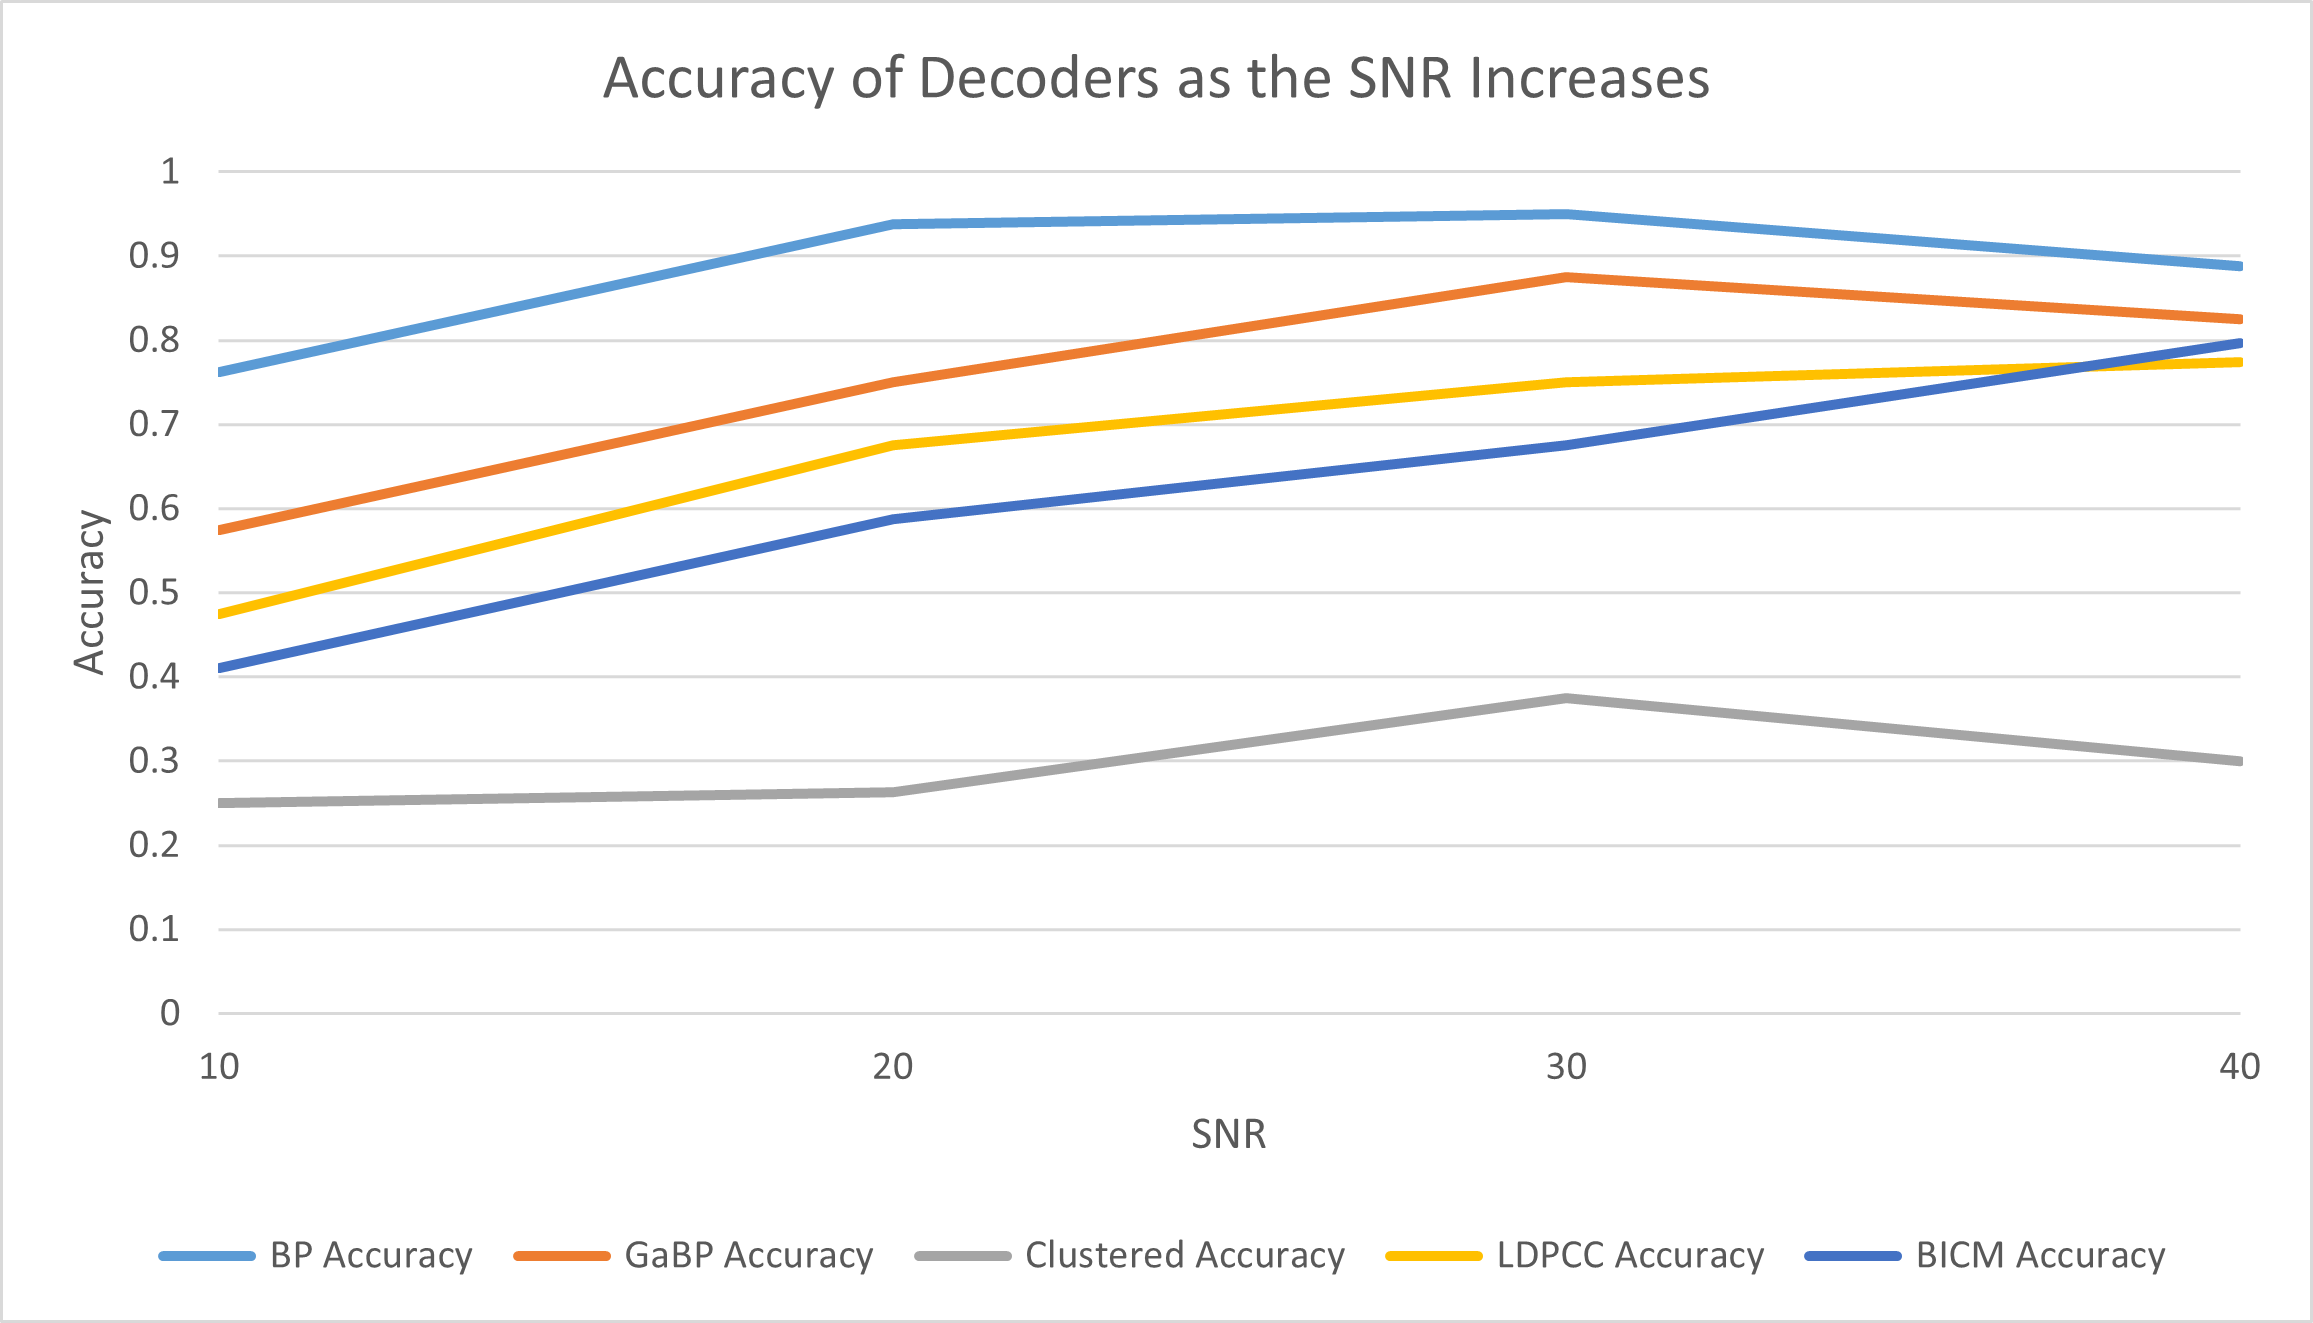
\includegraphics[width=0.30\textwidth]{SNRGraph.png}
    \caption{A comparison of the accuracy of the various decoders as the SNR increases.}
    \label{fig:SNRGraph}
\end{figure}

\section{Discussion}
The results show a couple core ideas. First of all, no particular system prefers or dislikes any variable over any other. However, we see a clear weakness in the clustered approximation. This is actually somewhat expected, as in a proper experiment, the size of the clusters would be adjusted to compare results. However, to be able to compare every algorithm in every setting, it would have been infeasible to also compare to every cluster size or every iteration count of every algorithm as well. Lastly, the LDPCC accuracy and BICM accuracy and not particularly favorable, mostly because the simulation only properly decodes them rarely, and spends an eternity coputing otherwise. This is completely due to experimental error, as the entire framework for this experiment was conducted on each following decoder being able to be modularly added, and thus was not expected systems like LPDCC and BICM. The code was written following guides that treated them individually, which is not proper, and given more time and resources the framework of the simulation should have been overhauled to allow them to be properly demonstrated. It also would have been preferred to run these simulation on larger values, but that was limited by the weak hardware used to run the simulation.

\end{document}